\addtocontents{toc}{\protect\newpage}
\section{Simulation Results}
\label{sec:results}

\subsection{Baseline Scenario}
\label{sec:baselinesc}

The model with the described implementation has been tested on the Sioux-16 network
with a flow capacity scaling of $70\%$ to allow for a reasonable amount of congestion.

The travel disutility parameter has been chosen to be zero, as is the travel
disutility for taking a car in Sioux-16. The reason behind this is that there are
numerous studies indicating positive and negative effects of autonomous vehicles, so
it is hard to decide whether the perception of AVs will tend towards one side or the
other compared to cars.

The constant disutility for cars in the Sioux-14 scenario
has been computed by combining the travel disutility for 10min walking (as to
account for getting to and from a parking lot) and the monetary disutility for
paying \$6 for parking. For the AVs in this simulation it has been assumed that
there is no such additional cost, but a monetary fee per AV trip. This
assumes that a fictitious operator already included the costs of parking into the
pricing scheme (which is reasonable taking the values from actual taxi services).

Since the values in Sioux-14 are based on measurements in Sydney, the current
maximum charges for taxi trips there have been used as a reference \citep{NSW2016}. According to this
source, an initial charge of \$3.60 has been set as the constant disutility per trip, while
the monetary distance factor for AVs has been set to \$2.19 per km.

Finally, the disutility for waiting for an AV has been assumed to be the same as
the waiting disutility for public transport from Sioux-14, which itself is just a
vague assumption \citep{Chakirov2014}, but at least allows for a systematic comparison.

\begin{table}[]
\centering
\caption{Baseline Scenario Parameters}
\label{tab:baselineparams}
\begin{tabular}{@{}lll@{}}
\toprule
Parameter                       & Computation & Baseline Value \\ \midrule
Constant Utility per Trip       & $C_{av} = -\beta_m \cdot \$3.60$    & $-0.2232$ \\
Marginal Utility of Travel Time & $\beta_{trav,av} = \beta_{trav,car}$            & $0.0$ \\
Monetary Distance Rate          & $\gamma_{car} = 2.19 \$/km$            &  $0.00219$              \\
\midrule
Marginal Utility of Wait Time   & $\beta_{wait,av} = \beta_{wait,pt}$            &  $-0.18$              \\ \bottomrule
\end{tabular}
\end{table}

Using these parameters, which are summarized in \cref{tab:baselineparams}, the
scenario has been simulated until relaxation. The following paragraphs will show
the respective results in terms of the traffic situation. A sufficiently high
number of available AVs ($N=8000$) has been chosen to show how agents make a choice for taking
an AV based on their utility evaluation.

\subsubsection{Trip Statistics}

\Cref{tab:withwithoutav} shows the basic trip statistics of the case where
AVs have been introduced to the baseline scenario. It can be seen that with the
given utility parameters, the AVs reach a share of around $25\%$ averaged over
the day, mainly decreasing the share of public transport and walking while also
attracting some of the former private car users.

Interesting to see is that for public transport and walking agents the travel
distances decreases because relatively long trips in those modes will be replaced
by AVs, thus drawing the average down to shorter trips, while it increases for cars.
Here, mainly the shorter car trips are replaced by AVs.

These results can also be in \cref{fig:modehist_av}, where the distribution of
travel distances by mode is presented. Clearly, AVs act as a competitor towards
public transport there, serving mainly the same range of trips with the assumed
utility parameters.

\begin{figure}
    \centering
    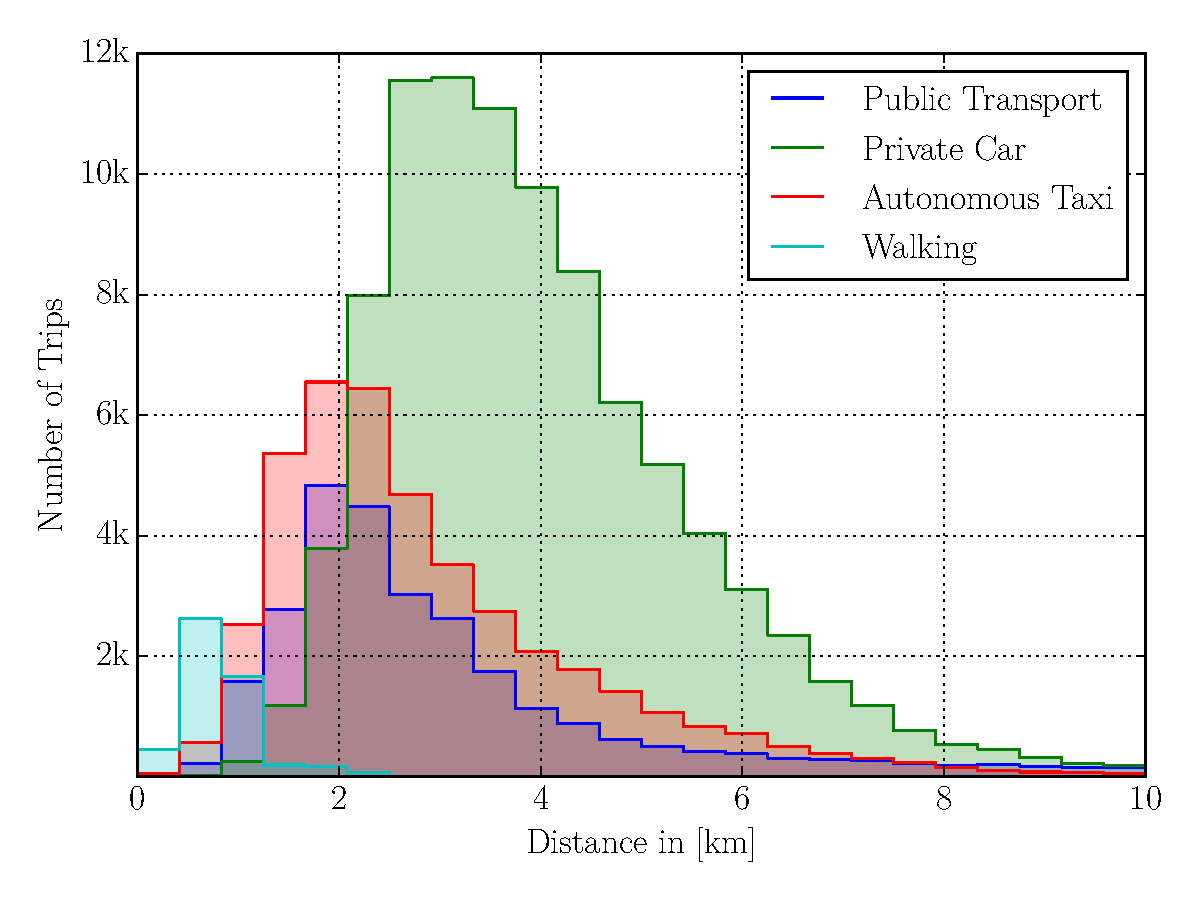
\includegraphics[width=0.85\textwidth]{figures/modehist_av.pdf}
    \caption{Number of trips for each node by traveled distance}
    \label{fig:modehist_av}
\end{figure}

In terms of travel times, it can be seen that there is a slight increase for the car
mode, which stems from the same argument as before. The decrease in travel time for
public transport and walking agents is quite significant, though. For the walking
agents, the change is obvious as described before. The decrease for public transport
can be explained by the switch of agents, who needed to have long walking distances
to the closest bus stop, which is included in the calculation. By only keeping those
agents at using public transport, who live nearby a bus stop, the overall travel
time decreases quite substantially.

% Please add the following required packages to your document preamble:
% \usepackage{booktabs}
\begin{table}[]
\centering
\caption{Traffic measures for the relaxed AV baseline scenario}
\label{tab:withwithoutav}
\begin{tabular}{@{}lll@{}}
\toprule
                                   & \textbf{Baseline} & \textbf{With AV} \\ \midrule
\textbf{Travel Distances {[}km{]}} &                   &                  \\
Car                                & 3.73              & 4.04             \\
Walking                            & 1.25              & 0.82             \\
Public Transport                   & 3.88              & 3.25             \\
Autonomous Taxi                    &                   & 2.94             \\
\textbf{Travel Times {[}mm:ss{]}}  &                   &                  \\
Car                                & 07:20             & 08:07            \\
Walking                            & 25:01             & 16:29            \\
Public Transport                   & 28:48             & 20:41            \\
Autonomous Taxi                    &                   & 10:41            \\
\textbf{Mode Shares}               &                   &                  \\
Car                                & 65.04\%           & 55.08\%          \\
Walking                            & 6.79\%            & 3.08\%           \\
Public Transport                   & 28.17\%           & 16.65\%          \\
Autonomous Taxi                    &                   & 25.19\%          \\ \bottomrule
\end{tabular}
\end{table}

The waiting times for AVs in the baseline scenario are on average around 04:40 min in the morning peak
and 02:55 min in the afternoon, while the daily average lies at 01:40 min. A more
detailed analysis of waiting times is given in \cref{sec:waitingtimes}.

In terms of travel distances the total amount of kilometers driven increased from around 424,000 km in
the baseline to 553,000 km in the AV scenario. The amount of kilometers driven by AVs
is 162,500 km from which around 37,800 are for the purpose of picking up passengers, i.e.
they are unoccupied while covering this distance, which is roughly $23\%$. This is around half
compared to ordinary taxis with 52\% as stated in recent statistics for Oslo \citep{Norway2015}
or around 50\% in Barcelona \citep{Amat2014}.

\subsubsection{Mode Choice}

\Cref{tab:basemodeshares} shows how the mode choice that takes place after AVs
have are introduced. The rows show the original modes while the percentages
indicate how many of the initial users switch to the mode in the column after the
introduction of AVs. What can be seen is that $44\%$ of all initial public transport
users and $56\%$ of all walking people opted for taking an AV while only $14\%$
of car users switch modes. This again shows that with the baseline parameters, AVs rather
work as a competitor against public transport while additionally drawing new adopters
from the walking people. Therefore, this scenario represents the rather unwanted case
where AVs lead to a less optimal situation on the road, leading to more
congestion and less use of collective transportation.

% Please add the following required packages to your document preamble:
% \usepackage{booktabs}
\begin{table}[]
\centering
\caption{Migration matrix showing which agents switched from one mode to another:
The rows resemble the initial choices of the agents while the columns resemble the
mode choice after the introduction of AVs. The percentages denoted how many users
of the original mode switched to another option.}
\label{tab:basemodeshares}
\begin{tabular}{@{}lrrrr@{}}
\toprule
                 & AV & Car     & PT & Walking \\ \midrule
Car              & 13.69\%    & 84.41\% & 1.68\%           & 0.23\%  \\
Public Transport & 44.29\%    & 0.60\%  & 54.91\%          & 0.21\%  \\
Walking          & 56.21\%    & 0.18\%  & 1.38\%           & 42.24\% \\ \bottomrule
\end{tabular}
\end{table}

A further impression on the choice behavior of the agents can be obtained through
\cref{fig:changes_modes}. In the upper plot one can see the public transport trips
in the baseline without AVs (blue), which have not changes during the introduction
of the new mode while the red dots show those combinations of trip duration and
distance in the original scenario, which have changed to AV. Comparing the blue
and red areas it becomes evident that users with rather long trips in terms of
travel time switch to AVs. The green dots show the combinations after the change
has been taken place, i.e. the travel duration and distance in the converted AV
trips. It can be seen that after the introduction of AVs the travel durations
get much less, so for the public transport users, the AV mode is mainly attractive
because it provides shorter net travel durations.

The lower plot in \cref{fig:changes_modes} shows the same arrangement for private
car users. One can see that the switching users (red) are clustered for short trips in
distance and duration. Their travel times, contrary to the public transport users,
increase when using the AVs, indicating that the monetary benefit of using the AV
instead of going on a private car trip (and paying for parking) is stronger than
the desire to have a minimal travel time.


\begin{figure}
    \centering
    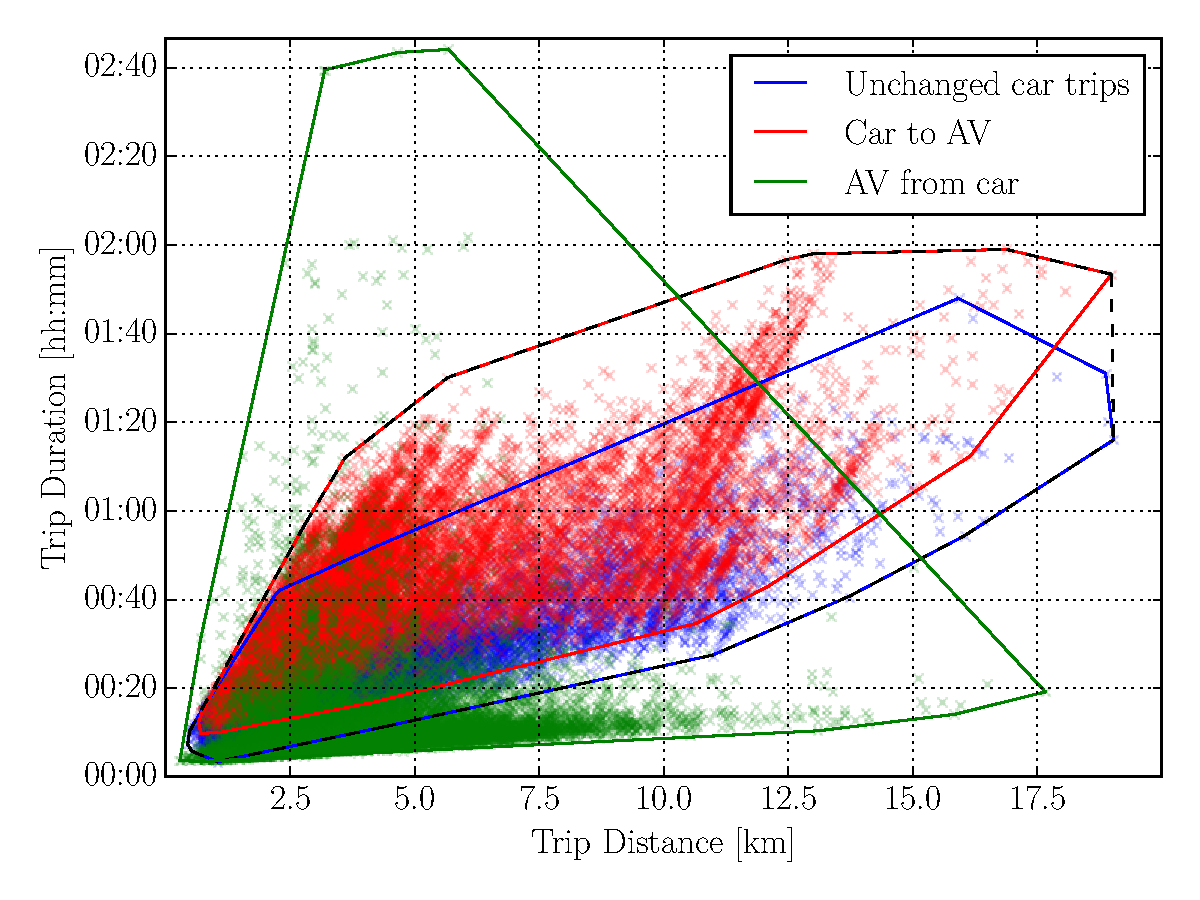
\includegraphics[width=0.85\textwidth]{figures/changes_pt.pdf}
    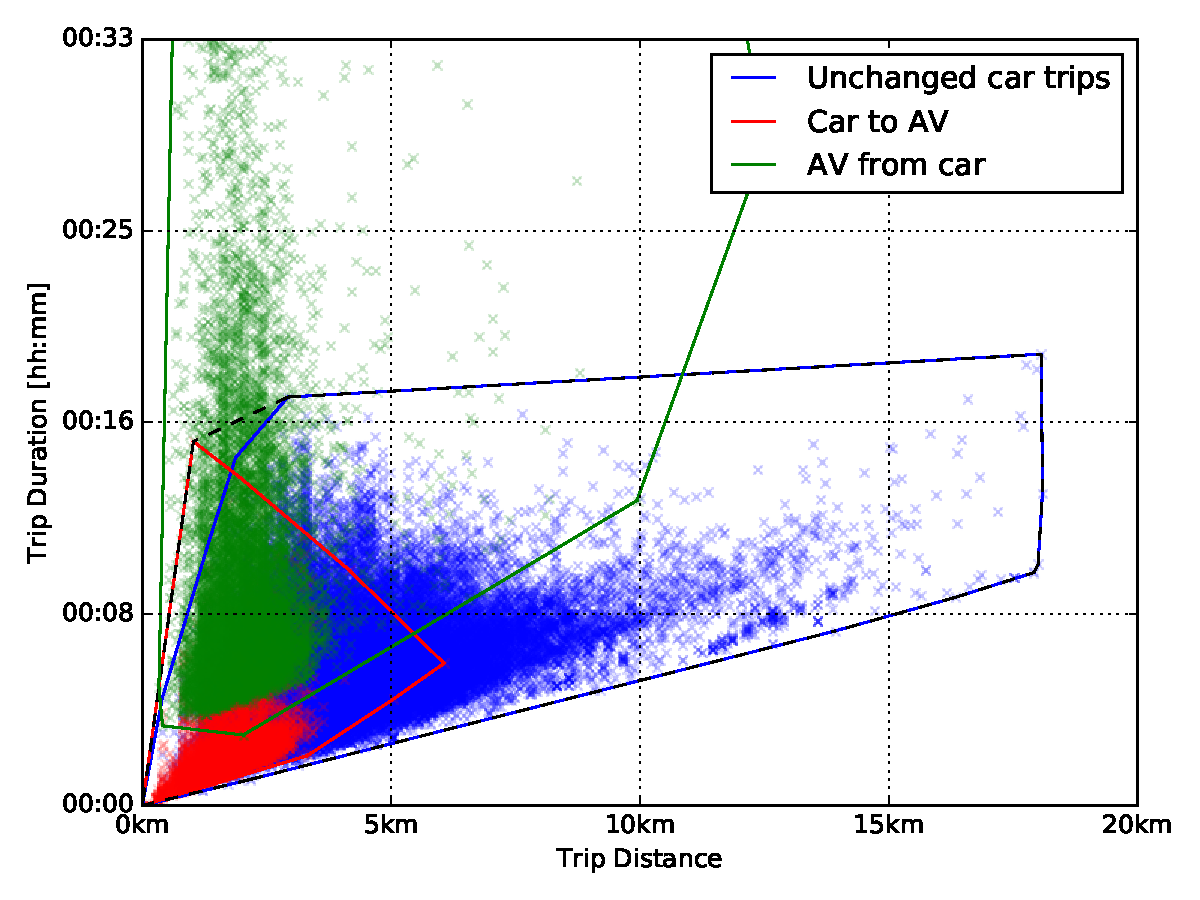
\includegraphics[width=0.85\textwidth]{figures/changes_car.pdf}
    \caption{Analysis of the distribution of public transport (top) and car (bottom) trips
    in terms of travel distance and duration before and after the introduction of
    autonomous vehicles.}
    \label{fig:changes_modes}
\end{figure}

\subsubsection{AV Operation and decreased supply}

Finally, \cref{fig:avwork} shows the states of the AVs during the day. While the
lines show how many AVs are currently performing either a pickup or dropoff task,
i.e. being ``en tour'', the shaded areas show how many passengers have been picked
up or dropped off at a certain time of the day. In this baseline scenario, only
around 3000 cars are actually active of the available 8000, so from the perspective
of an AV operator the scenario would not be an ideal case, because the
usage of the AVs is not nearly close to saturation.

\begin{figure}
    \centering
    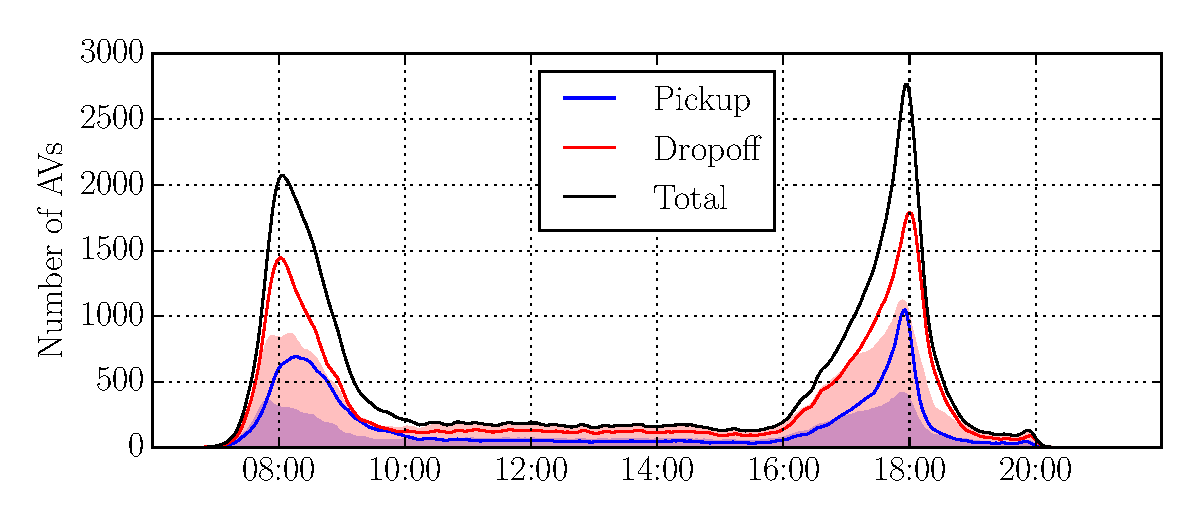
\includegraphics[width=1.0\textwidth]{figures/avwork.pdf}
    \caption{Activities of AVs during the day in the relaxed (8000 AVs) AV baseline scenario.
    The solid graphs show the number of vehicles, which are ``on tour'', while the
    shaded area denotes the number of pickup and dropoff interactions with the
    passenger.}
    \label{fig:avwork}
\end{figure}

Such a case is depicted in \cref{fig:avwork_low}. It shows the states of the AVs during the day
if only 1000 of them are available. Shaded areas
indicate those times of the day where the dispatchment mode changes from
oversupply to undersupply, where there are more requests than available AVs. At those
peak times, one
can see that the number of active AVs goes into saturation. The number does not
go to 1000 exactly since only driving AVs are measured, whereas some might be in
the 120s pickup or 60s dropoff activities.

\begin{figure}
    \centering
    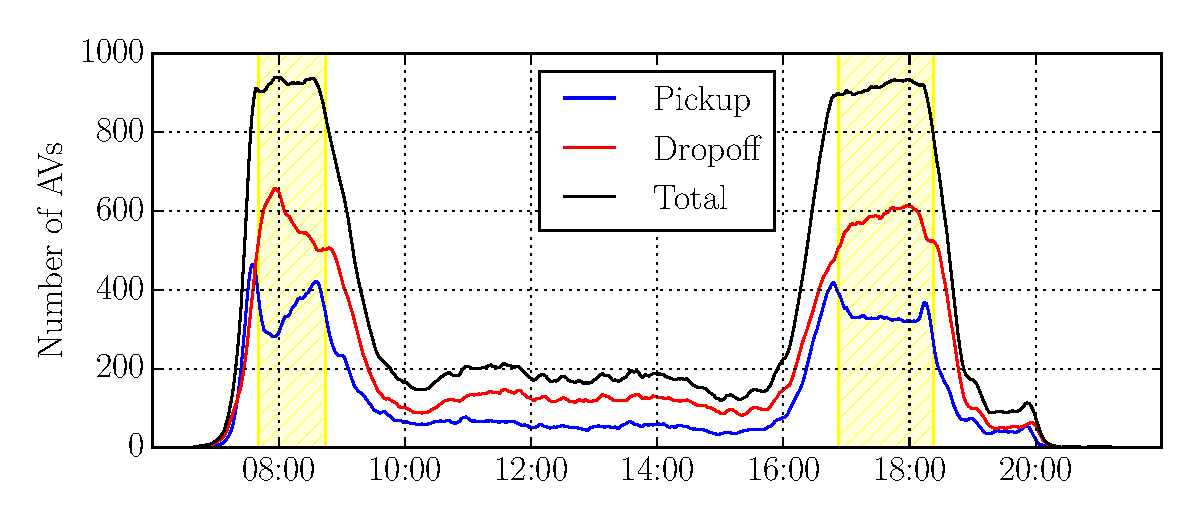
\includegraphics[width=1.0\textwidth]{figures/avwork_low.pdf}
    \caption{Activities of AVs during the day in the constrained (1000 AVs) AV baseline scenario.
    The show the number of vehicles, which are ``on tour'', while the
    shaded area denotes times where the undersupply dispatchment mode is active.}
    \label{fig:avwork_low}
\end{figure}

Compared to the high supply case, the share of AV trips drops from 25.19\% to
18.92\%. While the travel time stays roughly the same for the AV mode, the
average distance increases slightly from 2.94km to 3.18km, indicating a shortfall
of short trips. Around half the amount of private car users
switch to AVs (6.65\%, before 13.69\%); for public transport users, the decrease
is less significant from 44.29\% to 40.29\%. From that one can conclude that the
attractiveness of AVs for private car users is decreasing substantially with a
constrained supply while the induced longer waiting times seem to be tolerable
by former public transport users.

\begin{figure}
    \centering
    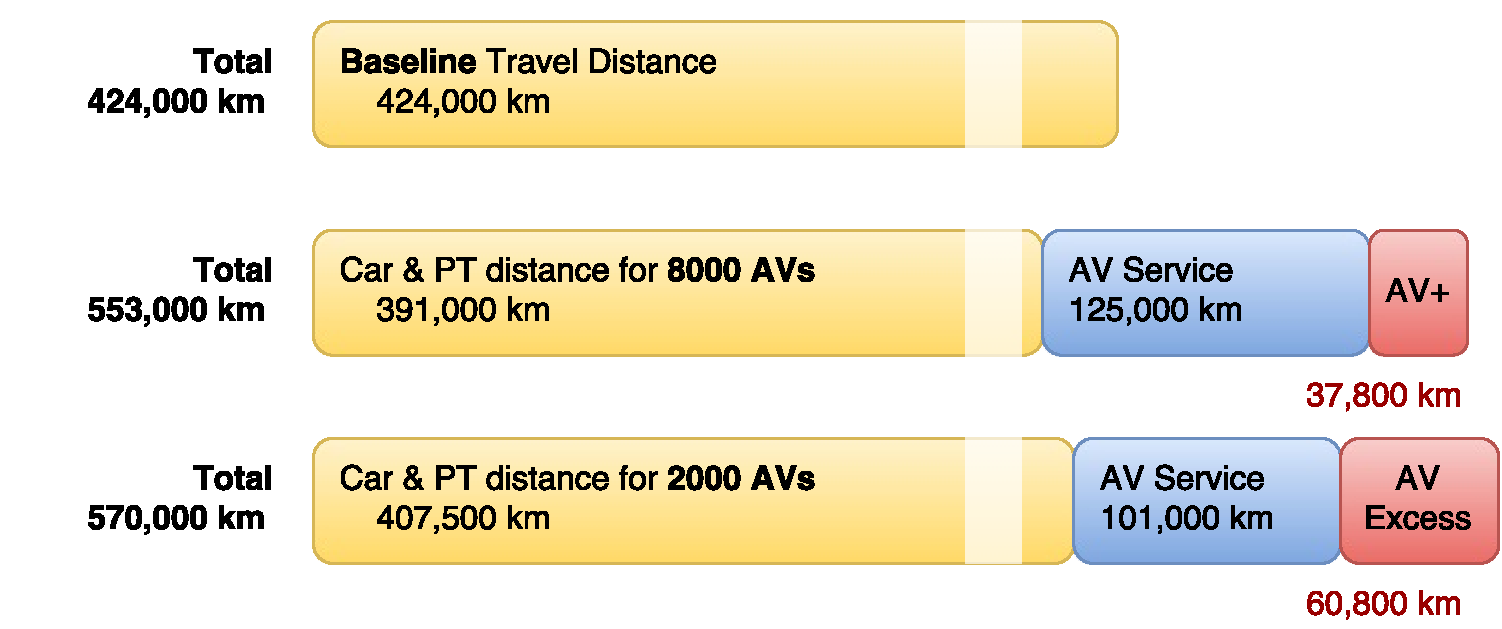
\includegraphics[width=1.0\textwidth]{figures/traveldistances.pdf}
    \caption{Comparison of total travel distances in the low and high supply scenarios.}
    \label{fig:traveldistances}
\end{figure}

From an environmental perspective, this scenario
is worse than the former one. While car users continue using their private vehicles,
public transport users switch to additional cars on the road. In terms of distance
(\cref{fig:traveldistances}), the total amount of kilometers driven increases further
because of an increase in excess travel distance of the AVs. Since fewer agents are
using the service, the vehicles have to cover longer distances to get to the next
customer. Such a case is disadvantageous for the service operator, so it will be
interesting to see how the additional costs of excess mileage affect the overall
economic evaluation of the provider (\cref{sec:economics}). The next chapter will
give a more detailed relation of the supply level on the total traveled distance.

\subsection{Supply Analysis}
\label{sec:waitingtimes}

\Cref{fig:excessdistance} shows the relation of travel distance and supply in
a more detailed way. At around 1000 vehicles, there is a peak of the net driven
distance in the network (black), which is relaxed if the supply is increased. The
stable added number of kilometers is then around 120,000km. However, the peak is
only 40,000km bigger than this value, which itself is a quarter of the initial
400,000km in the base scenario. Looking at the red graph, which shows the added
miles of empty drives in the AV services compared as an offset to the total number
of AV miles, one can see that it shows the same peak, i.e. the excess mileage is
responsible for the increase in total travel distance. In this regard, the service
operator and public administration would have the same priority to avoid this peak
(in terms of profit one one side and regarding environmental policy and congestion on the other).

\begin{figure}
    \centering
    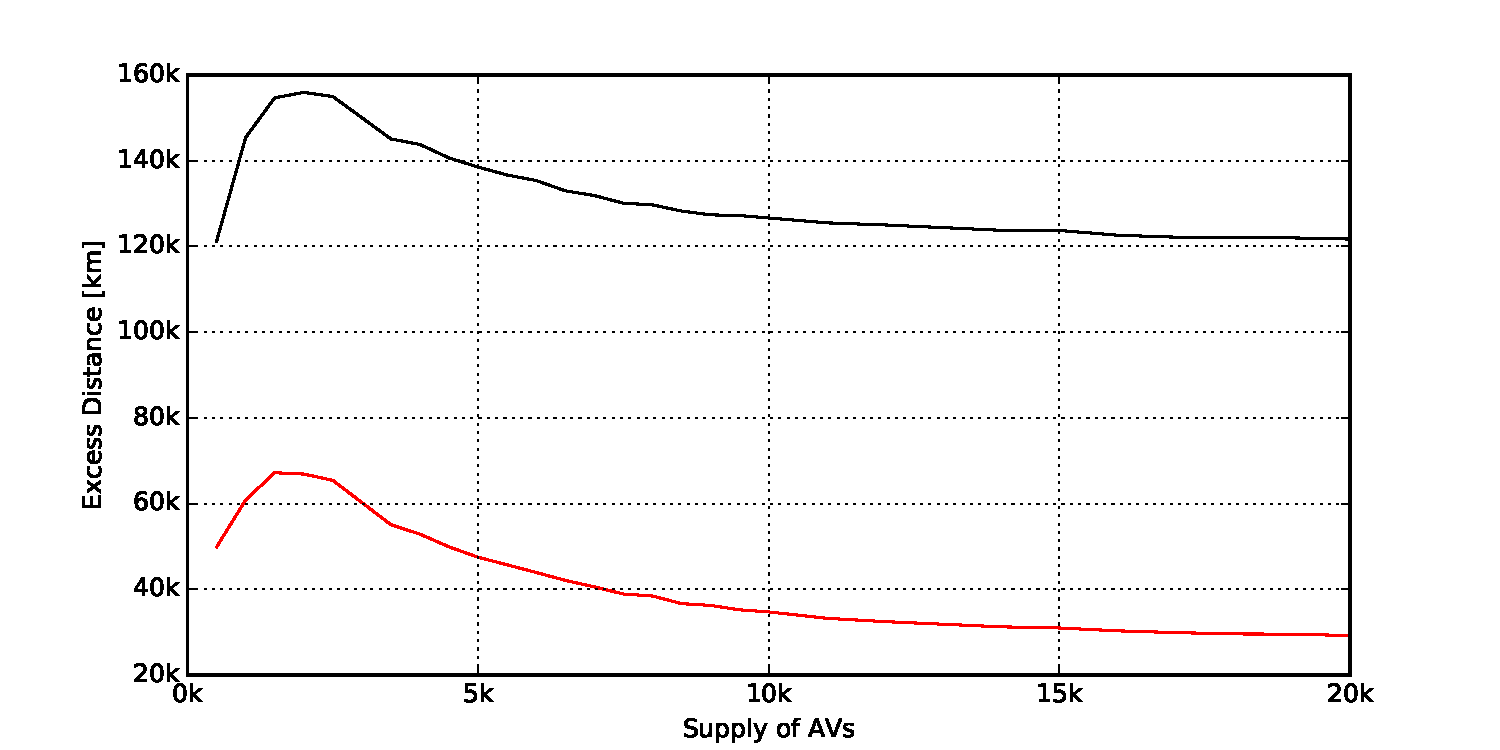
\includegraphics[width=1.0\textwidth]{figures/excessdistance.pdf}
    \caption{Evaluation of the total added travel distance of all vehicles compared
    to the base scenario without AVs (black) and excess driving distance for AVs
    for the respective supply (red).}
    \label{fig:excessdistance}
\end{figure}

In terms of waiting time it has been found that per 1000 AVs around 4\% of
initial car trips in the scenario could be replaced with static demand in \cref{sec:replacement}.
Looking at the waiting times on top in \cref{fig:waitingsupply}
one can see that the mean value as well as the 90\% quantile of the waiting time
$t_W$ is under the threshold of 10 minutes, which has been examined before. Furthermore, the middle of
\cref{fig:waitingsupply} shows $P(t_W \leq 10 min)$, i.e. the probability of having
a waiting time of less than 10 min in the simulated supply scenarios. While this
probability clearly decreases with small fleet sizes, it still stays rather high
at 90\%. That is the case, because due to high waiting times, fewer trips are being
made. For higher supplies, the quantile finds an equilibrium-like state at around
97\%, which can be interpreted as a measure of how tolerable increased waiting times are
in a certain scenario.

Additionally, the bottom plot in \cref{fig:waitingsupply} shows the replaced
percentage of trips dependent on the amount of available AVs. Because of the
preferences that are induced through the utility-based learning, considerably
fewer trips are converted to AVs although staying in the waiting time limits.
While in the static analysis 5000 AVs can replace 20\% of private car trips,
in the dynamic one it is only 15\%. For the static case 60\% are simulated
at 15,000 AVs, but here the replacement fraction remains at 15\%. This shows
that the usefulness of the mode, which is quantified by the utility, is the
restricting factor, despite a large available margin in waiting time efficiency.

\begin{figure}
    \centering
    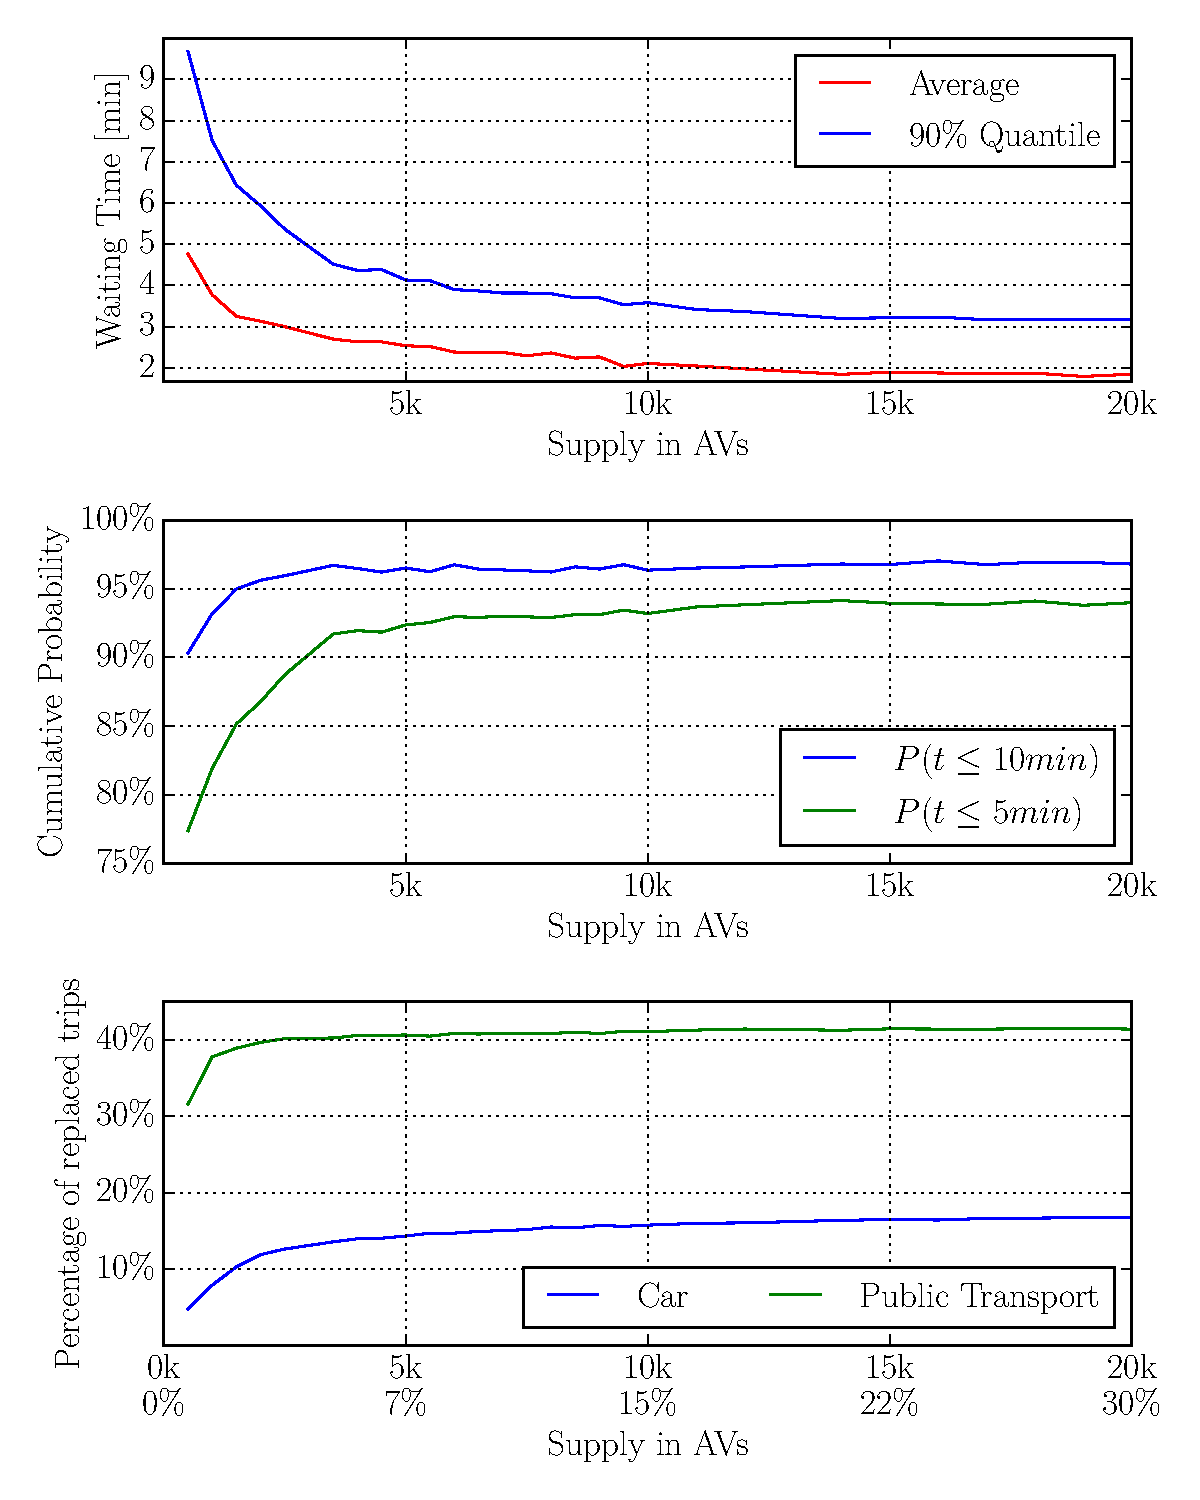
\includegraphics[width=1.0\textwidth]{figures/waitingsupply.pdf}
    \caption{Top: Mean value and 90\% quantile of waiting time for different supply
    levels. Bottom: Cumulative probability of observing a waiting time less than
    10 minutes.}
    \label{fig:waitingsupply}
\end{figure}

\subsection{Cost Dependencies}
\label{sec:costs}

Intuitively, the behavior of the utility parameters should be quite clear: If
the utility is increased, the AV mode gets more favorable, if it is decreased, less
people will use it. However, in such a complex traffic system there are secondary
effects, which influence the adaptation of AVs.

\Cref{fig:sharegrid} shows the share of the AV mode in the baseline scenario (top)
with different pricing schemes, given through a price per kilometer and a price
per trip. For very cheap services, the share reaches 90\%, while for a combination
of \$7 per trip and \$3 per kilometer the share drops down to under 10\%. It can
be seen that for a very low travel utility (lower left) the threshold in the shares
gets steeper while it dilutes for  very high travel utility (i.e. acceptance)
of the AV mode (lower right). This hints at the fact that the more accepted AV
technology is in the population, the more people will use it while the pricing
scheme can have a huge impact on adaptation if there is a considerable amount of
skepticism towards the technology.

\begin{figure}
    \centering
    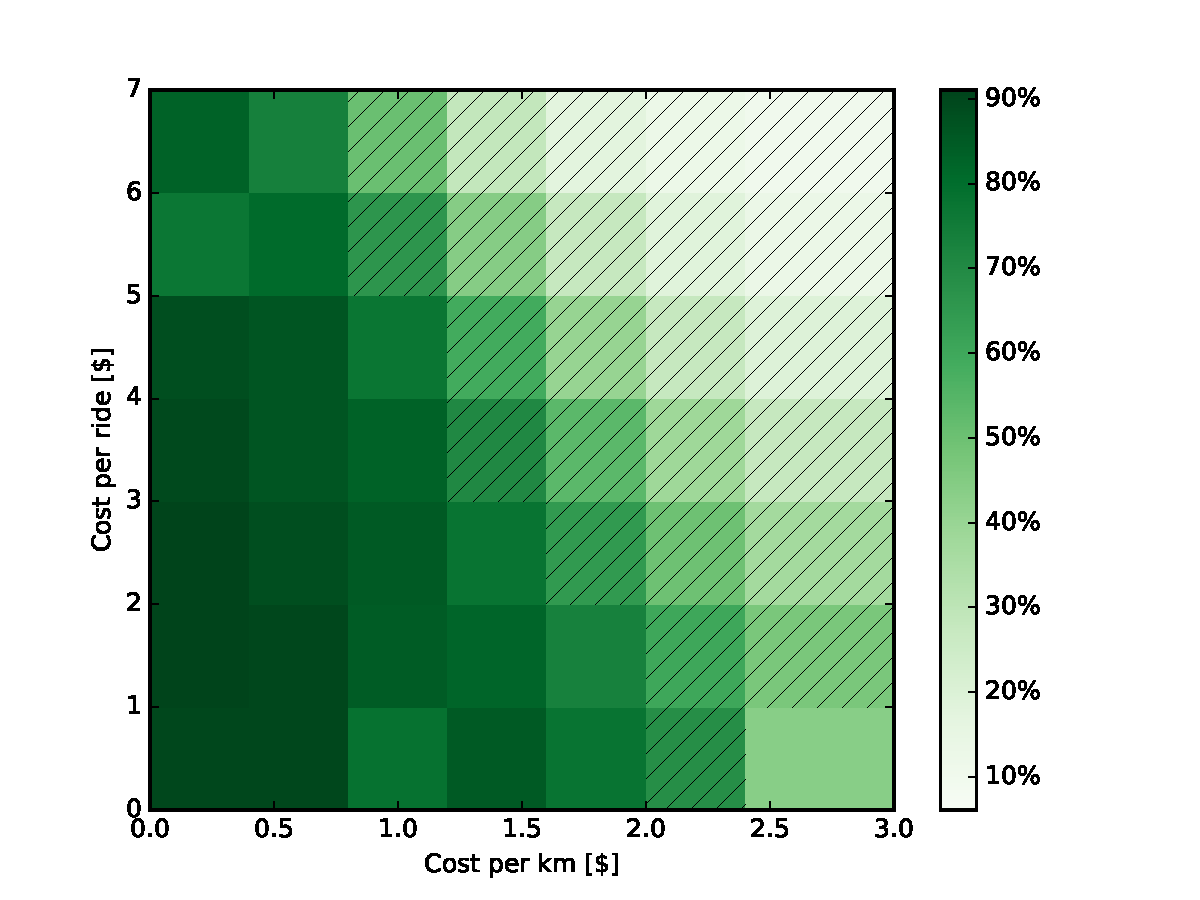
\includegraphics[width=0.8\textwidth]{figures/sharegrid.pdf}
    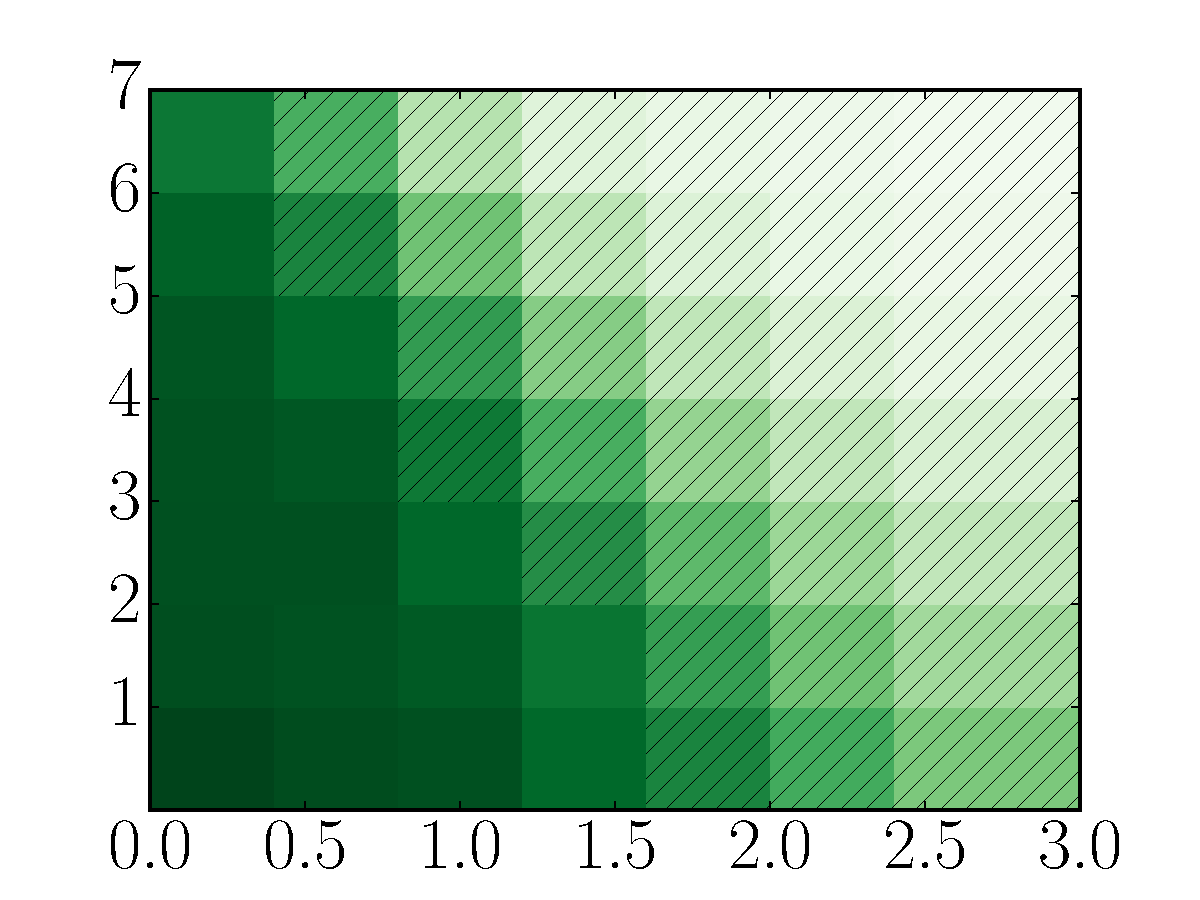
\includegraphics[width=0.45\textwidth]{figures/sharegrid_n05.pdf}
    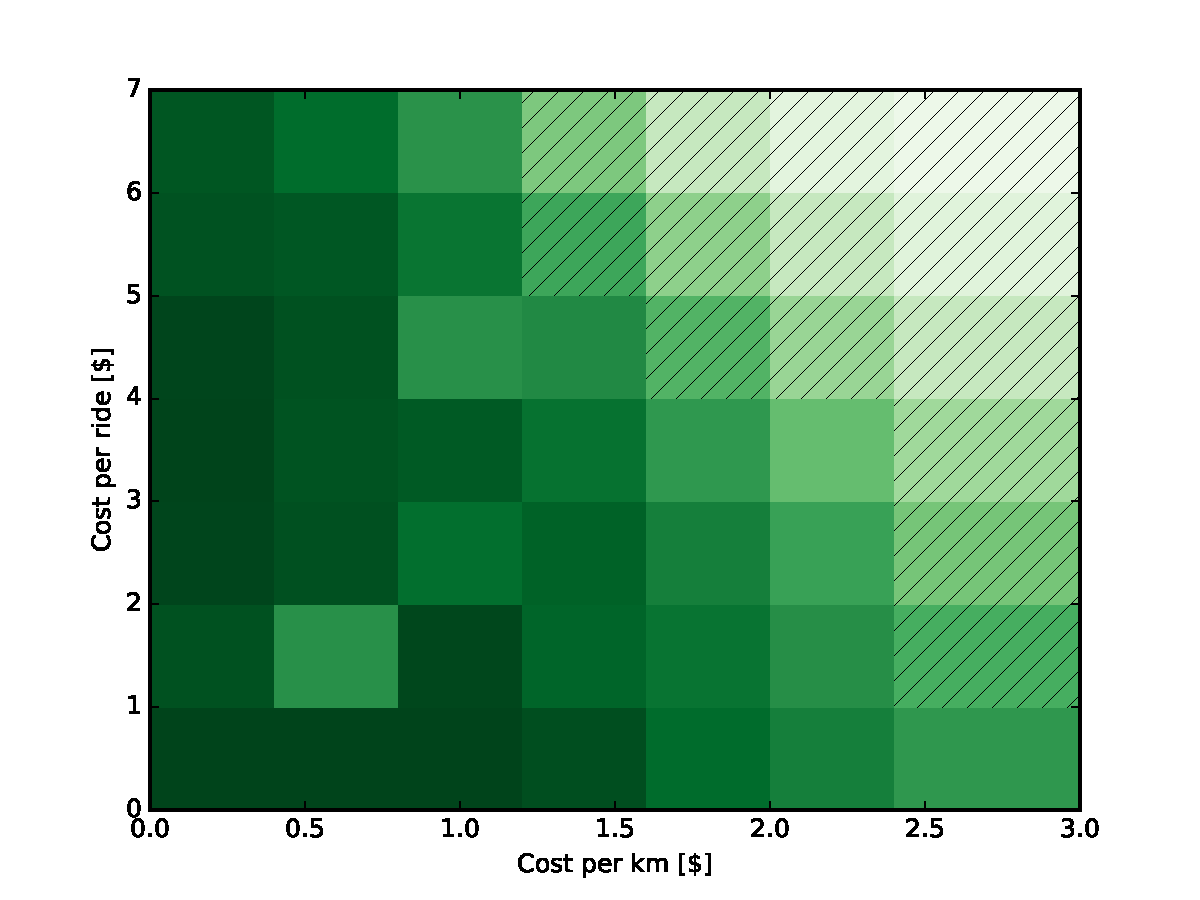
\includegraphics[width=0.45\textwidth]{figures/sharegrid_p05.pdf}
    \caption{Dependency of the AV mode share on the pricing scheme. Top: Baseline
    scenario. Left: Low utility of traveling ($\beta_{trav,av} = -0.5$). Right: High utility
    of traveling ($\beta_{trav,av} = 0.5$). Shaded areas show parameter combinations
    where the waiting time for an AV is shorter than 10 min in 90\% of the cases.}
    \label{fig:sharegrid}
\end{figure}

The shaded areas in \cref{fig:sharegrid} show those parameter combinations, where
$P(t_w \leq 10min) \geq 0.9$, i.e. where the probability to wait less than 10
minutes for an AV per trip is higher than 90\%. Taking that as another criterion
to assess the performance of an AV service, one can see that it puts a restriction
on how low the prices can drop to allow for a smooth operation of the
service. In fact, if waiting time is a constraint, only moderate shares of AVs
can be reached on any level of acceptance.

What needs to be kept in mind here is that no further investigations on the
disutility of waiting time have been performed here, but it is rather based on an
assumption taken from \citet{Chakirov2014}. Nonetheless, the result is surprising
since, in extreme cases, agents accept a waiting time of 30 minutes or more in
90\% of trips, as can be seen on top in \cref{fig:moregrids}. Mainly, this depends
on all the utility parameters in the scenario, also the utility of performing an
activity, the disutility of using other means of transport and so forth. Accepting
such a high waiting time might be an indicator that the utilities in the Sioux
scenario should be further improved to lead to better results. However, the interpretation
is tricky for very low prices, since they also resemble quite unrealistic situations, where
only times are weighed against each other: If there are no monetary costs, a trip
in terms of utility costs as much as not performing an activity for the travel time.

Furthermore, the results of the simulation are surprising when looking at the share
of public transport on the bottom in \cref{fig:moregrids}. The general tendency makes
sense: Lower prices lead to lower shares of public transport because using an AV
gets more advantageous. Also, having very high prices, the public transport share
stays at its initial baseline level. Nevertheless, one would expect people to
react more abrupt to the pricing scheme on the per-trip side than on the per-km
side. So far each trip in the Sioux Falls scenario costs \$2. Imposing no per-trip
fee for AVs, but different per-km fares should show a smooth transition as can be seen
in \cref{fig:moregrids}: The shares
should change depending on the price and the trip distance distribution.
On the other hand, if no per-km fare is imposed, but only per-trip payments, the
transition should be more abrupt. This effect, however, might be smoothed out by
AVs taking less travel time.

This is only true though if people can make rational decisions about the
total costs of travel. When looking at the beforementioned plots, one can see
that there is are quite linear nivau lines, meaning that if a per-km cost is given,
one can easily obtain the per-trip cost in order to stay at a certain level of
service. For instance, this means that for the agents, paying \$5 per trip and
\$1.60 per km is equal to paying \$3 per trip and \$1.90 per distance. In reality, the perception of the high per-trip fare might be different to the lower
per-km fare, especially compared to the initial \$2 per trip.

\begin{figure}
    \centering
    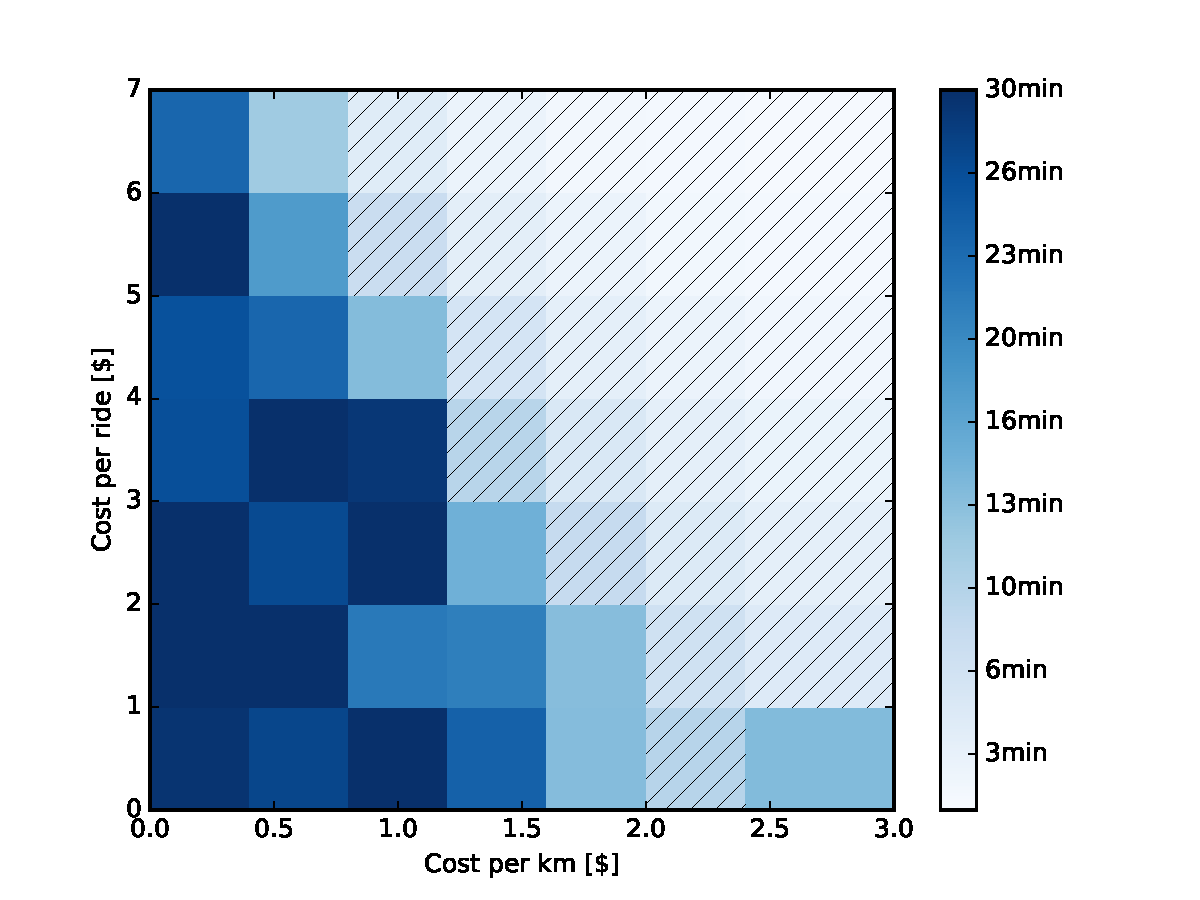
\includegraphics[width=0.7\textwidth]{figures/waitingtimegrid.pdf}
    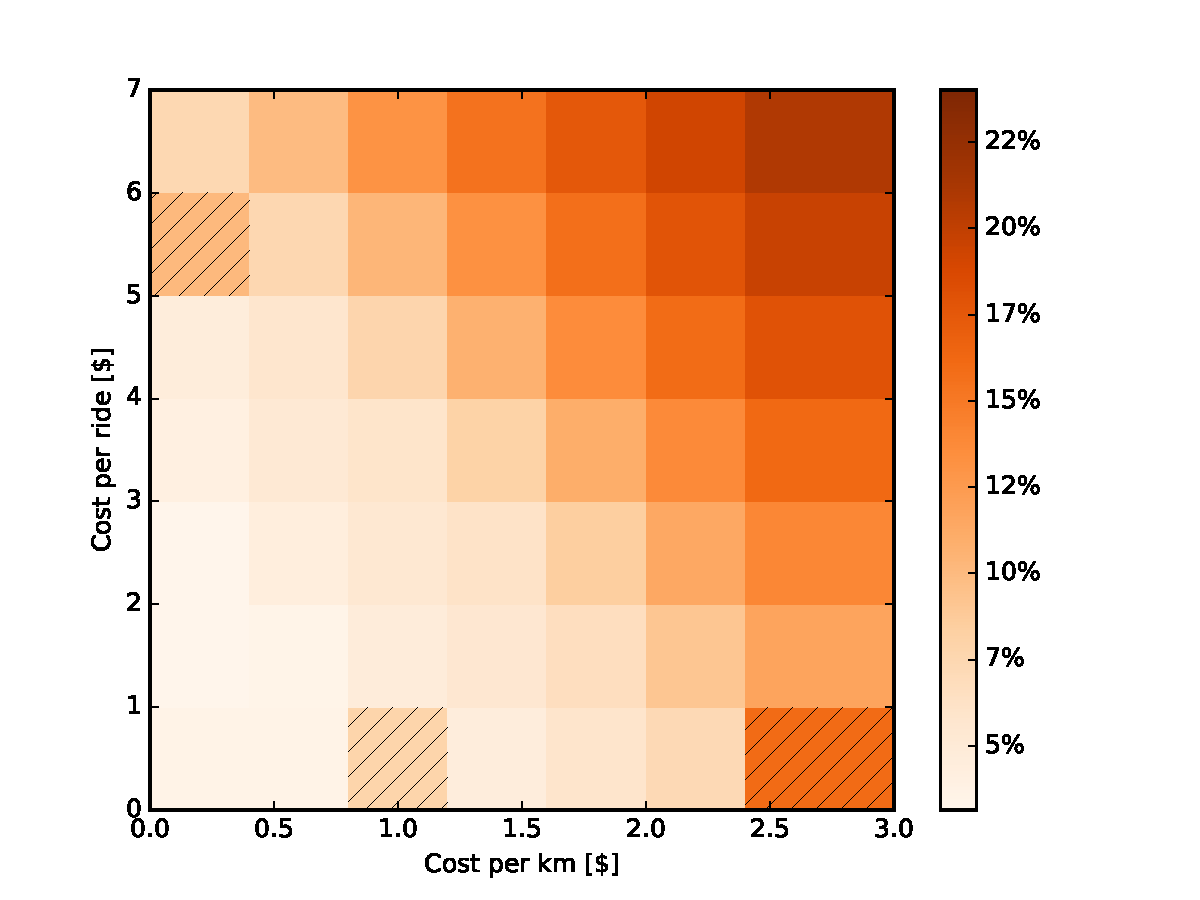
\includegraphics[width=0.7\textwidth]{figures/ptsharegrid.pdf}
    \caption{Top: 90\% quantile of the waiting time in the baseline scenario with different
    pricing schemes. The scale is truncated at 30 minutes. Bottom: Share of public transport
    trips. Shaded areas indicate not completely relaxed simulation runs with stuck agents.}
    \label{fig:moregrids}
\end{figure}

Combining the results of this section, it becomes apprent that in the given scenario,
also the share of public transport has a lower bound if a specific service level in
terms of waiting time should be maintained. On the other hand, the introduction of
AV services will diminish the share of public transport in any case. As one conclusion
it can be therefore stated that without any policy-based incentives, it is not possible
to maintain the level of public transport while motivating private car owners to switch to AVs.

Another point that has to be taken into account regarding these considerations is
the profitability of the service for the operator, which will be the subject of the
next section.

\subsection{Economical Analysis}
\label{sec:economics}

The operator model for the net income $z$ proposed in this thesis can be stated as follows:

\begin{equation}\begin{aligned}
z
&= \underbrace{p_{km} \cdot d_{dropoff} + p_{trip} \cdot n_{trips}}_{Gross Income}\\
&- \left( \underbrace{\$6 \cdot n_{veh} + c_{pd} \cdot n_{veh} + \gamma_{d,car} \cdot d_{total}}_{Expenses} \right)
\label{eq:step1}
\end{aligned}\end{equation}

On the income side of the operator, there is the total distance of dropoff (i.e.
occupied) trips $d_{dropoff}$, multiplied by the price per km and the number
of AV trips $n_{trips}$, multiplied by the price per trip. The expense side has
been modeled to be comparable with the car mode in the Sioux-16 scenario. It involves
a cost for parking (\$6) as well as running costs per km for private cars multiplied by the combined
total distance for pickup and dropoff trips. Of course, this choice bears a lot
of uncertainty, it might be a reasonable guess though, since increased costs for
insurance and decreased costs for (electric) operational costs might weigh out
each other \citep{Chen15}. Finally, a cost per day
$c_{pd}$ is introduced for each supplied AV taxi.

That cost has been modeled as follows: \Citet{Chen15} states predictions of
(electric) AV taxi prices of around $c_{veh} = \$62,000$ (converted to AUD) and states lifetimes
of around $d_{max} = 370,000 km$. From the simulation the average driven distance
of one day is known as $d_{avg} = d_{total} / n_{veh}$ per vehicle. Those values can
be used to obtain a vehicle lifetime, assuming that the amount of kilometers
driven stays constant over the lifetime $\tau$:

\begin{equation}
\tau = \frac{d_{avg}}{d_{total} / 1d} = \left[ \frac{km}{km/d} \right] = [d]
\end{equation}

Then the costs per vehicle per day can be stated as:

\begin{equation}\begin{aligned}
c_{pd} &= \frac{c_{veh}}{\tau} = d_{avg} \cdot \frac{c_{veh}}{d_{max}} \\
&= d_{avg} \cdot \nu\\
&= \nu \cdot \frac{d_{total}}{n_{veh}}
\end{aligned}\end{equation}

with

\begin{equation}
\nu = 0.17 \frac{\$}{km}.
\end{equation}

Inserting this equation into \cref{eq:step1} effectively cancels out the number
of available AVs from the investment costs and integrates them into the per
distance costs:

\begin{equation}\begin{aligned}
z
&= \underbrace{p_{km} \cdot d_{dropoff} + p_{trip} \cdot n_{trips}}_{Gross Income}\\
&- \left( \underbrace{\$6 \cdot n_{veh} + (\nu + \gamma_{d,car}) \cdot d_{total}}_{Expenses} \right)
\label{eq:step1}
\end{aligned}\end{equation}

Therefore the net income is characterized by a complex relation of the total distance
driven, the occupied distance, the number of cars and the number of AV trips. Applying
this model to the previously introduced pricing scheme map gives the result in
\cref{fig:netincomegrid}. For very low prices the service clearly is not profitable
in the proposed model, while it is possible to maintain the service in a moderate
price range. In fact, the area with most profit is covered by the formerly introduced
condition on waiting times (hatched area). However, if a share of 15\% of public
transport share should be maintained, the operator would need to offer the service
in the crossed area. There the profit is decreasing because of a smaller
number of users.

For the baseline scenario, the operator scenario has been tested with different
supply levels. The results in \cref{fig:revenuesupply} show that over the whole
range of AVs there the service is profitable, especially at 4000 AVs. Over the whole
depicted range the constraints on waiting time and public transport are fulfilled.
In that sense those scenarios are quite optimal cases, where the share of
public transport stays above 15\%, the waiting times are usually less than 10
minutes and the operator has a large margin. Incorporating the results from
\cref{sec:baselinesc}, the right-most cases are the best because additionally
the overall excess mileage is smallest.

The large margin is an indicator that the baseline scenario is a setup
that could ``work'' in a city similar to the Sioux Falls network. Contrary to
the financial analysis in \Citet{Chen15}, here infrastructure costs have not been
included in the analysis, which could be covered by that profit of the operator.

\begin{figure}
    \centering
    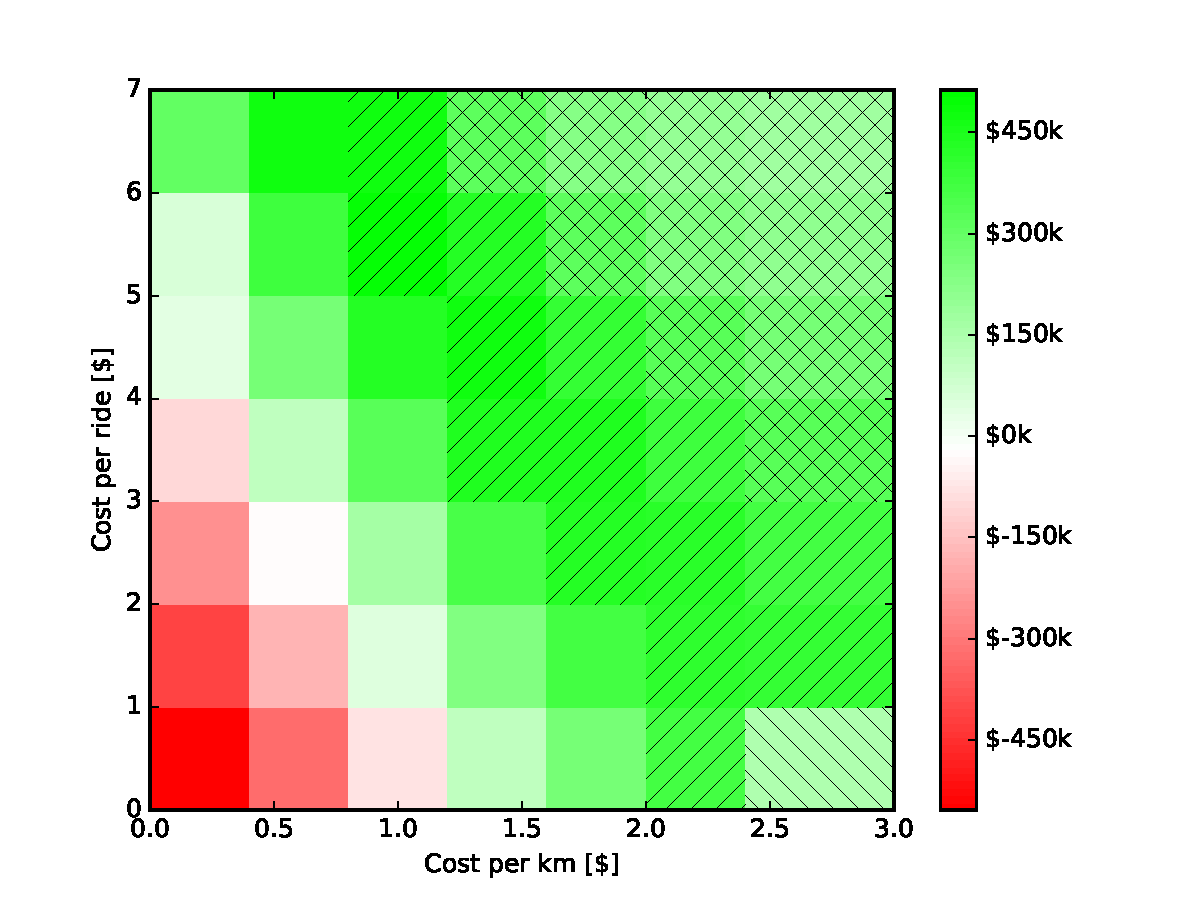
\includegraphics[width=0.85\textwidth]{figures/netincomegrid.pdf}
    \caption{Net income of the AV operator. The shaded areas represent acceptable
    waiting times (bigger area) and public transport mode shares of more than
    15\% (smaller area).}
    \label{fig:netincomegrid}
\end{figure}

\begin{figure}
    \centering
    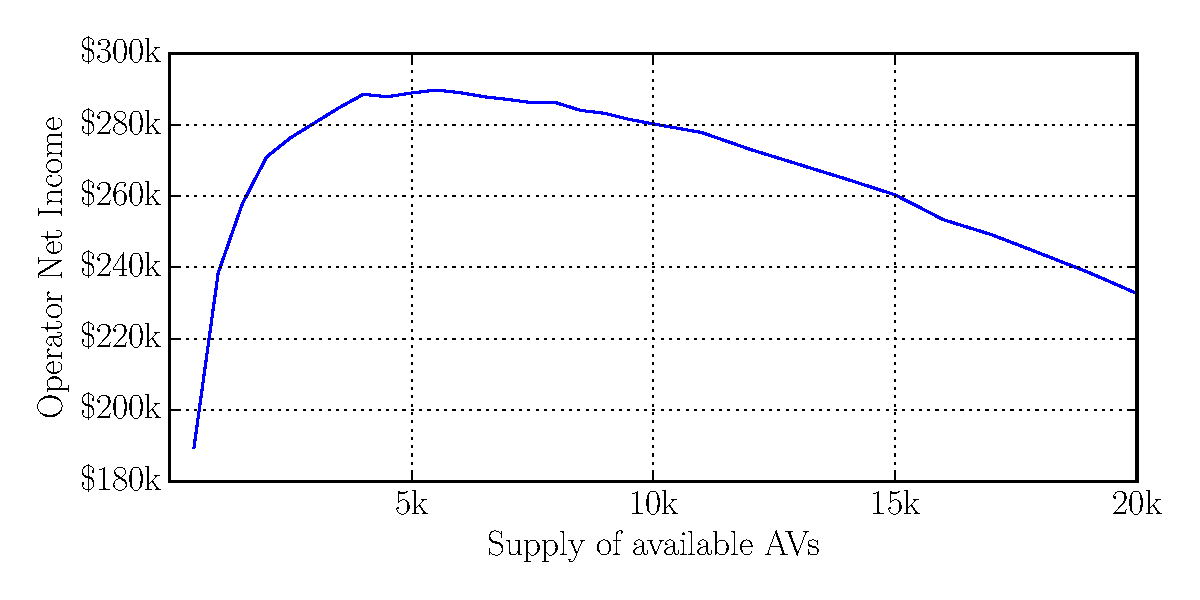
\includegraphics[width=1.0\textwidth]{figures/revenuesupply.pdf}
    \caption{Dependency of the operator net income in the baseline scenario on
    the number of supplied AVs.}
    \label{fig:revenuesupply}
\end{figure}

\subsection{Summary}

In the previous chapters the quantitative results of the AV simulation have been
demonstrated in detail. However, the simulation at hand is by nature more suited
for giving qualitative insights into the traffic system rather then quantitative
since it is based on a virtual test scenario. The following paragraphs will
summarize the beforementioned results and give a qualitative overview of the
findings, putting a focus on the main subject of the thesis: The interaction of
the new travel mode with the established means of transport.

One of the first results, which could be obtained, is that AVs in the test
scenario will lead to an increased overall milage, which is an adverse effect
looking from an environmentally perspective, but is also disadvantageous in
terms of congestion in the network. Implementation-wise it has been found that
considerable work needs to be put into intelligent ways of making AVs facilitate
the existing infrastructure in order to avoid artificially made traffic jams,
which is a problem that gets crucial with an increasing number of AV trips
and therefore increasing mileage.

In that regard the introduction of AVs plays against one positive effect of
public transport: to have fewer vehicles one the road. As could be shown in the
results, former public transport users are the main adapters of autonomous vehicles
in the given scenario. While private car users have a financial motivation to switch
to the AV mode and accept longer travel times, public transport users mainly do
the switch to reduce their accumulated travel time consisting of the walking
to the stop facilities and the ride itself, possibly with several line switches.

This choice behavior goes along with a high tolerance for waiting times for the
AV mode. Because public transport users are used to having a long travel time,
the performance that could be reached in the given network was clearly enough
to serve the demand. Nevertheless, the public transport users are not the
audience that a policy maker would want to attract with AVs. From the findings
in the simulations one can state (at least for the Sioux network), that it is
very hard to impossible to maintain a certain level of public transport while
getting private car owners to using the AV service. In fact, applying pinpointed
incentive or taxation schemes to the network might be necessary to reach at the
desired results.

In terms of pricing it has been found that the more inclined people are to spend
time in an AV, the less constrained the financial structure of the service needs
to be in order to reach certain AV shares. For the baseline scenario it has been
found that it is possible to operate an AV service in a profitable way while still
maintaining a share of \%15 public transport and providing waiting times of less
than ten minutes. While doing this, there would be a financial margin available
on the side of the operator to cover necessary infrastructural expenses.

The final conclusion is that AVs without administrative regulation are likely to
attract public transport users rather than private car owners. Further research
needs to be done on how AV usage can be incentivized for private car owners to
reach at a beneficial traffic situation.

Finally, it remains to state that the proposed model is built on a manifold of
assumptions in the initial Sioux Falls scenario, in the operation of the AV
agents and on the financial model for the operator. While for the latter future
predictions will become better and better, it would be highly interesting to apply
the developed model to a real-world scenario with a higher confidence in the estimated
utility parameters and relative factors such as current taxi pricing.
